\chapter{Mapas conformes y prescripción de dispersión de cuerdas abiertas}

\lectureoverview{Los mapas conformes aparecen primero como una simetría práctica de la electrostática bidimensional. La diferenciabilidad compleja convierte esa simetría en algo calculable: las ecuaciones de Cauchy--Riemann implican la ecuación de Laplace, y una derivada compleja independiente de la dirección conserva los ángulos. Con estas herramientas, una hoja de universo de cuerda puede representarse como una franja, un semiplano, un cilindro o un disco sin que cambie la física. La dispersión de cuerdas abiertas se convierte entonces en una integral de camino gaussiana sobre el disco, con inserciones de momento en su frontera, seguida de una integral sobre sus posiciones no equivalentes.}

\section{Electrostática en un mundo bidimensional}

Empezamos con un problema electrostático estrictamente bidimensional. Las cargas y sus líneas de campo están confinadas a un plano; no son simplemente cargas ordinarias tridimensionales cuyo movimiento resulta ser plano. La ley de Gauss da entonces
\begin{equation}
  F(r)\propto \frac{1}{r},
  \qquad
  V(r)\propto \log r,
  \label{eq:l08-two-dimensional-coulomb}
\end{equation}
porque el flujo atraviesa un círculo cuya circunferencia crece como \(r\).

Escribamos el campo en términos de un potencial escalar \(\phi\). Con la convención de signos usada en la pizarra,
\begin{equation}
  \mathbf E=\nabla\phi,
  \qquad
  \nabla\cdot\mathbf E=\rho,
\end{equation}
y, por tanto,
\begin{equation}
  \nabla^2\phi
  =\frac{\partial^2\phi}{\partial x^2}
  +\frac{\partial^2\phi}{\partial y^2}
  =\rho.
  \label{eq:l08-poisson}
\end{equation}
En una región sin cargas, esto se reduce a la ecuación de Laplace,
\begin{equation}
  \nabla^2\phi=0.
  \label{eq:l08-laplace-phi}
\end{equation}
\editorialnote{En muchos textos de electrodinámica se define
\(\mathbf E=-\nabla\Phi\), en cuyo caso
\(\nabla^2\Phi=-\rho\) una vez absorbidas las constantes. En la clase se usa el signo opuesto para el potencial. La ecuación sin fuentes y todos los argumentos conformes siguen siendo los mismos.}

\begin{figure}[H]
  \centering
  \includegraphics[width=0.72\textwidth]{lecture_08_figure_01.png}
  \caption{Las ecuaciones electrostáticas desplegadas como el operador de Poisson bidimensional.}
  \lectureframe{00:03:48}
  \label{fig:l08-electrostatics-board}
\end{figure}

El signo más entre las dos derivadas espaciales es importante. Hace que esta sea una ecuación elíptica, no una ecuación de ondas. Las transformaciones conformes preservan su forma sin fuentes, de modo que una solución en un dominio puede trasladarse a otro de forma distinta junto con sus condiciones de contorno. Esto resulta útil en electrostática, en el flujo de fluidos bidimensional y en cartografía, antes de serlo en teoría de cuerdas.

\begin{classroomqa}
\audiencequestion{Si el laplaciano se anula, ¿es esta una ecuación de ondas estacionarias? \lecturetimestamp{00:05:35}}
\lecturerresponse{No. Las dos derivadas espaciales tienen el mismo signo y no hay derivada temporal. Una ecuación de ondas requiere dependencia temporal con el signo relativo lorentziano. La electrostática es estática precisamente porque nada evoluciona, ni siquiera una onda.}
\end{classroomqa}

\begin{classroomqa}
\audiencequestion{¿Hay rotacional en dos dimensiones?
\lecturetimestamp{00:06:06}}
\lecturerresponse{Sí, pero solo tiene una componente independiente. Para
\(\mathbf E=(E_x,E_y)\),
\[
  \operatorname{curl}_{2d}\mathbf E
  =\partial_yE_x-\partial_xE_y.
\]
Puede imaginarse como la componente perpendicular a la pizarra, aunque un mundo intrínsecamente bidimensional no necesita ninguna dirección perpendicular externa. En dimensiones superiores, el objeto correspondiente es, de manera natural, una 2-forma antisimétrica.}
\end{classroomqa}

\section{Una derivada sin dirección preferente}

Introduzcamos coordenadas complejas en los planos original y de imagen:
\begin{equation}
  z=x+iy,
  \qquad
  w=u+iv,
  \qquad
  w=w(z).
  \label{eq:l08-complex-coordinates}
\end{equation}
Aquí \(x,y,u,v\) son reales. Localmente, la derivada debería ser
\begin{equation}
  \frac{dw}{dz}
  =\lim_{\Delta z\to0}\frac{\Delta w}{\Delta z}.
  \label{eq:l08-complex-derivative}
\end{equation}
A diferencia de la recta real, el plano complejo admite infinitas direcciones de aproximación. Una aplicación continua y normalmente suave no tiene por qué dar la misma razón en todas ellas.

Comparemos dos aproximaciones sencillas. En la dirección \(x\), \(dy=0\), así que
\begin{equation}
  \left.\frac{dw}{dz}\right|_x
  =\frac{\partial u}{\partial x}
  +i\frac{\partial v}{\partial x}.
\end{equation}
En la dirección \(y\), \(dx=0\), y
\begin{equation}
  \left.\frac{dw}{dz}\right|_y
  =\frac{1}{i}\frac{\partial u}{\partial y}
  +\frac{\partial v}{\partial y}
  =\frac{\partial v}{\partial y}
  -i\frac{\partial u}{\partial y}.
\end{equation}
La igualdad de las partes real e imaginaria da
\begin{equation}
  \boxed{
  \frac{\partial u}{\partial x}
  =\frac{\partial v}{\partial y},
  \qquad
  \frac{\partial u}{\partial y}
  =-\frac{\partial v}{\partial x}}
  \label{eq:l08-cauchy-riemann}
\end{equation}
Estas son las ecuaciones de Cauchy--Riemann. Bajo los supuestos habituales de diferenciabilidad, también bastan para que el límite
\eqref{eq:l08-complex-derivative} sea independiente de la dirección. Una función con esta propiedad es analítica, u holomorfa, en ese punto.

\begin{figure}[H]
  \centering
  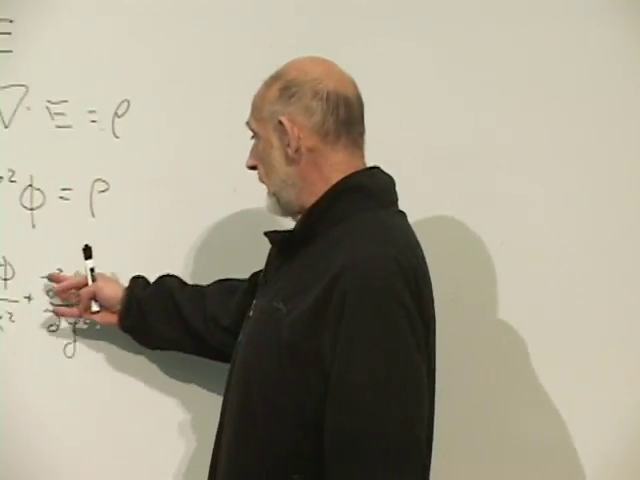
\includegraphics[width=0.70\textwidth]{lecture_08_figure_02.png}
  \caption{El par completo de Cauchy--Riemann, incluido el signo relativo negativo.}
  \lectureframe{00:19:48}
  \label{fig:l08-cr-board}
\end{figure}

La clase distingue brevemente términos relacionados. Una función holomorfa en todo el plano complejo finito es entera. Una función meromorfa puede tener polos aislados. Así, \(1/z\) es analítica salvo en \(z=0\), pero no es entera.

\section{Conjugadas armónicas y geometría conforme}

Las ecuaciones de Cauchy--Riemann son ecuaciones acopladas de primer orden, pero implican ecuaciones separadas de segundo orden. Derivemos \(\partial_xu=\partial_yv\) respecto de \(x\), derivemos \(\partial_yu=-\partial_xv\) respecto de \(y\) y sumemos:
\begin{align}
  \partial_x^2u&=\partial_x\partial_yv,\\
  \partial_y^2u&=-\partial_y\partial_xv,\\
  \therefore\qquad
  \partial_x^2u+\partial_y^2u&=0.
  \label{eq:l08-harmonic-u}
\end{align}
Repitiendo el argumento con \(u\) y \(v\) intercambiadas, se obtiene
\begin{equation}
  \partial_x^2v+\partial_y^2v=0.
  \label{eq:l08-harmonic-v}
\end{equation}
Por tanto, las partes real e imaginaria de una función analítica son conjugadas armónicas. Dos funciones armónicas cualesquiera no forman automáticamente una función analítica: todavía deben estar relacionadas por \eqref{eq:l08-cauchy-riemann}.

\begin{figure}[H]
  \centering
  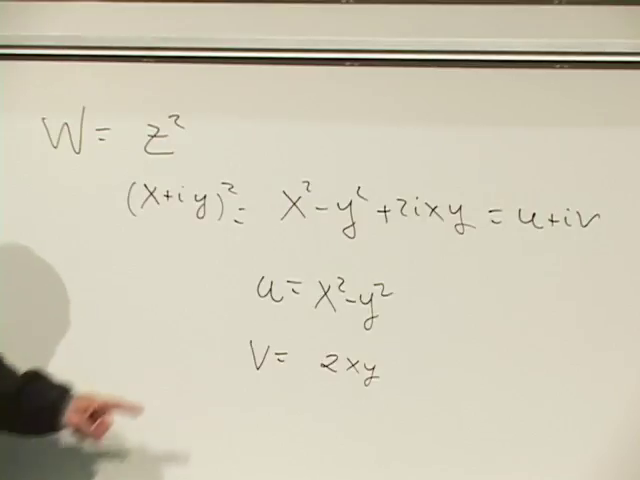
\includegraphics[width=0.68\textwidth]{lecture_08_figure_03.png}
  \caption{Las derivadas mixtas se cancelan y queda la ecuación de Laplace para una componente de la aplicación analítica.}
  \lectureframe{00:23:09}
  \label{fig:l08-harmonic-board}
\end{figure}

También hay una interpretación vectorial útil. Si
\(\mathbf F=(u,-v)\), las dos ecuaciones de Cauchy--Riemann indican, salvo por la convención de orientación elegida, que tanto la divergencia como el rotacional bidimensional de \(\mathbf F\) se anulan. Así volvemos a la electrostática, como se había anunciado.

\subsection{Por qué se conservan los ángulos}

Escribamos dos pequeños desplazamientos complejos en forma polar:
\begin{equation}
  \delta z=\rho e^{i\theta},
  \qquad
  \Delta z=\rho'e^{i\theta'}.
\end{equation}
La fase de su cociente es \(\theta-\theta'\), exactamente el ángulo entre ellos. Bajo una aplicación analítica,
\begin{equation}
  \frac{\delta w}{\delta z}
  =\frac{\Delta w}{\Delta z}
  =w'(z),
\end{equation}
porque la derivada no depende de la dirección. Reordenando, se obtiene
\begin{equation}
  \frac{\Delta z}{\delta z}
  =\frac{\Delta w}{\delta w}.
  \label{eq:l08-angle-ratio}
\end{equation}
Ambos lados tienen la misma fase, así que el ángulo entre los segmentos originales es igual al ángulo entre sus imágenes.

\begin{figure}[H]
  \centering
  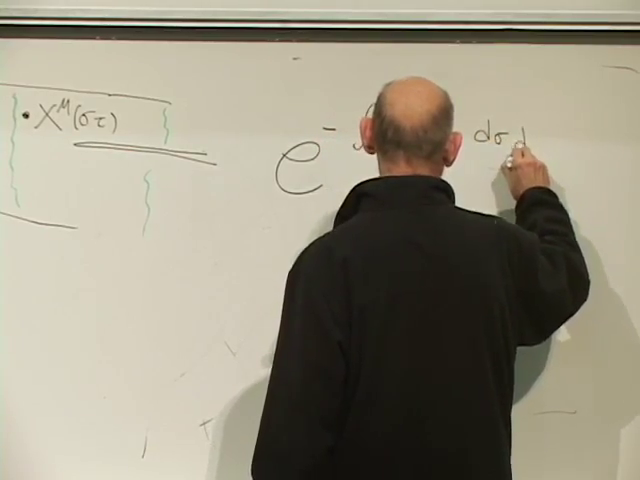
\includegraphics[width=0.70\textwidth]{lecture_08_figure_04.png}
  \medskip

  \begin{tikzpicture}[x=0.9cm,y=0.9cm,>=Latex]
    \begin{scope}
      \draw[->] (-0.2,0) -- (2.3,0);
      \draw[->] (0,-0.2) -- (0,2.1);
      \draw[very thick,blue!65!black,->] (0,0) -- (1.85,0.45)
        node[right] {\(\delta z\)};
      \draw[very thick,orange!75!black,->] (0,0) -- (0.72,1.65)
        node[above] {\(\Delta z\)};
      \draw (0.58,0.14) arc[start angle=14,end angle=66,radius=0.60];
      \node at (1.0,-0.55) {\(z\)-plane};
    \end{scope}
    \draw[->,thick] (3.0,0.9) -- (4.2,0.9)
      node[midway,above] {\(w(z)\)};
    \begin{scope}[xshift=5.0cm]
      \draw[->] (-0.2,0) -- (2.3,0);
      \draw[->] (0,-0.2) -- (0,2.1);
      \draw[very thick,blue!65!black,->] (0,0) -- (1.65,0.70)
        node[right] {\(\delta w\)};
      \draw[very thick,orange!75!black,->] (0,0) -- (0.48,1.62)
        node[above] {\(\Delta w\)};
      \draw (0.54,0.23) arc[start angle=23,end angle=74,radius=0.59];
      \node at (1.0,-0.55) {\(w\)-plane};
    \end{scope}
  \end{tikzpicture}
  \caption{La demostración de la pizarra y una reconstrucción local ordenada. La multiplicación por \(w'(z)\) hace girar y cambiar de escala todas las direcciones infinitesimales en la misma medida, preservando sus ángulos relativos.}
  \lectureframe{00:34:11}
  \label{fig:l08-angle-proof}
\end{figure}

Este argumento local supone que \(w'(z)\neq0\). En un punto crítico, la aplicación puede dejar de ser localmente biyectiva y hay que tratar la geometría por separado. Fuera de esos puntos, las aplicaciones analíticas y las aplicaciones conformes que preservan la orientación son localmente los mismos objetos.

\section{Ejemplos para entrenar la intuición}

\subsection{El cuadrado y la conjugación compleja}

Para \(w=z^2\),
\begin{equation}
  (x+iy)^2=x^2-y^2+2ixy=u+iv,
\end{equation}
por tanto,
\begin{equation}
  u=x^2-y^2,
  \qquad
  v=2xy.
  \label{eq:l08-z-squared-components}
\end{equation}
Las segundas derivadas de \(u\) son \(2\) y \(-2\); las de \(v\) se anulan por separado. Ambas funciones son armónicas, y la derivación directa también verifica las ecuaciones de Cauchy--Riemann.

\begin{figure}[H]
  \centering
  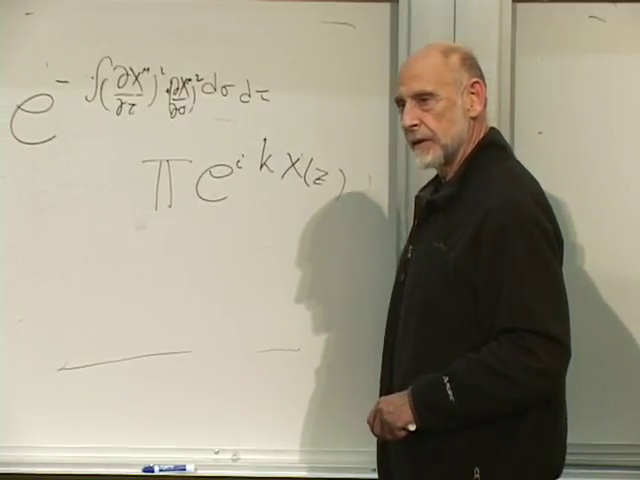
\includegraphics[width=0.72\textwidth]{lecture_08_figure_05.png}
  \caption{La aplicación cuadrática descompuesta en sus componentes armónicas real e imaginaria.}
  \lectureframe{00:36:45}
  \label{fig:l08-z-square-board}
\end{figure}

\begin{classroomqa}
\audiencequestion{¿Da \(1/z\) un ejemplo de función no analítica?
\lecturetimestamp{00:37:49}}
\lecturerresponse{Solo en un punto. Es analítica donde \(z\neq0\) y tiene un polo en el origen. Para ver una aplicación que no supere la prueba de Cauchy--Riemann en ningún punto, la conjugación compleja es un ejemplo más adecuado.}
\end{classroomqa}

En cambio,
\begin{equation}
  w=\bar z=x-iy
  \qquad\Longrightarrow\qquad
  u=x,\quad v=-y
\end{equation}
invierte la orientación. Sus derivadas incumplen por un signo la primera ecuación de Cauchy--Riemann, así que no es analítica como función de \(z\).

\begin{figure}[H]
  \centering
  \includegraphics[width=0.62\textwidth]{lecture_08_figure_06.png}
  \caption{La conjugación compleja ofrece el contraejemplo deliberadamente no analítico.}
  \lectureframe{00:38:38}
  \label{fig:l08-conjugate-board}
\end{figure}

\subsection{La exponencial y su inversa}

\begin{classroomqa}
\audiencequestion{Si \(e^z\) es analítica, ¿por qué también debería ser analítica su inversa \(\log z\)? \lecturetimestamp{00:40:38}}
\lecturerresponse{Donde existe la inversa y \(w'(z)\neq0\), su derivada es \(1/w'(z)\). Por tanto, se conserva la independencia respecto de la dirección. Globalmente, el logaritmo es multivaluado, así que se elige una rama y se excluyen su punto de ramificación y su corte. La afirmación local sobre la conformidad sigue siendo válida en el dominio elegido.}
\end{classroomqa}

La fórmula de Euler da
\begin{equation}
  w=e^z=e^{x+iy}
  =e^x(\cos y+i\sin y),
\end{equation}
y, por tanto,
\begin{equation}
  u=e^x\cos y,
  \qquad
  v=e^x\sin y.
  \label{eq:l08-exponential-components}
\end{equation}
Por ejemplo,
\(\partial_xu=e^x\cos y=\partial_yv\), y la segunda ecuación de Cauchy--Riemann se deduce con la misma facilidad.

\begin{figure}[H]
  \centering
  \includegraphics[width=0.68\textwidth]{lecture_08_figure_07.png}
  \caption{Las componentes real e imaginaria de la aplicación exponencial.}
  \lectureframe{00:42:23}
  \label{fig:l08-exponential-board}
\end{figure}

\section{Semiplano, franja, cilindro y disco}

\subsection{El logaritmo convierte el radio en tiempo}

Tomemos el semiplano derecho, donde
\(-\pi/2<\theta<\pi/2\), y escribamos
\begin{equation}
  z=re^{i\theta},
  \qquad
  w=\log z=\log r+i\theta.
  \label{eq:l08-log-map}
\end{equation}
El semiplano se transforma en la franja infinita
\begin{equation}
  -\frac{\pi}{2}<\operatorname{Im}w<\frac{\pi}{2}.
\end{equation}
Los rayos de \(\theta\) fijo se convierten en rectas horizontales, mientras que las semicircunferencias de \(r\) fijo se convierten en rectas verticales. El origen se transforma en \(\operatorname{Re}w=-\infty\), y \(r=\infty\) en \(\operatorname{Re}w=+\infty\).

\begin{figure}[H]
  \centering
  \includegraphics[width=0.75\textwidth]{lecture_08_figure_08.png}
  \caption{El logaritmo lleva el semiplano derecho a una franja infinita: los rayos polares y las semicircunferencias forman una cuadrícula rectangular ortogonal.}
  \lectureframe{00:47:48}
  \label{fig:l08-log-strip-board}
\end{figure}

La franja es la hoja de universo estándar de una cuerda abierta. Su coordenada acotada parametriza la cuerda, mientras que la traslación a lo largo de la dirección no acotada es el tiempo de la hoja de universo. Bajo la aplicación exponencial inversa, una traslación temporal se convierte en una dilatación \(z\mapsto e^a z\). Así, la misma simetría aparece como una traslación en la franja y como una expansión uniforme en el semiplano.

\begin{classroomqa}
\audiencequestion{¿Adónde va un valor particular como \(r=1\), y siguen siendo polares las coordenadas de la franja? \lecturetimestamp{00:50:58}}
\lecturerresponse{Un círculo de radio fijo se convierte en una recta vertical en \(\operatorname{Re}w=\log r\); en particular, \(r=1\) se transforma en la recta central \(\operatorname{Re}w=0\). Las coordenadas polares describen el plano \(z\). El plano \(w\) usa coordenadas rectangulares ordinarias \((\log r,\theta)\).}
\end{classroomqa}

Si se transforma todo el plano perforado mediante \(\log z\), la coordenada angular tiene período \(2\pi\). Por tanto, los bordes superior e inferior de la franja resultante quedan identificados: es un cilindro infinito. El semiplano con frontera describe la hoja de universo de una cuerda abierta; el plano completo, sin frontera y con ángulo periódico, describe un cilindro de cuerda cerrada.

\begin{figure}[H]
  \centering
  \includegraphics[width=0.75\textwidth]{lecture_08_figure_09.png}
  \caption{La representación del semiplano como franja y la identificación periódica que convierte el plano perforado completo en un cilindro de cuerda cerrada.}
  \lectureframe{00:54:23}
  \label{fig:l08-open-closed-board}
\end{figure}

\subsection{Una aplicación de Cayley al disco unidad}

Una aplicación fraccional lineal, o de Möbius, transforma el semiplano derecho en el disco unidad:
\begin{equation}
  w=\frac{z-1}{z+1}.
  \label{eq:l08-cayley}
\end{equation}
Envía \(z=0\) a \(-1\), \(z=\infty\) a \(+1\) y el eje imaginario a \(|w|=1\). Si \(z=ir\),
\begin{equation}
  \left|\frac{ir-1}{ir+1}\right|=1.
\end{equation}
Los puntos con \(\operatorname{Re}z>0\) quedan dentro del círculo; el semiplano izquierdo se transforma en el exterior.
\editorialnote{Durante la derivación en directo se escribe el recíproco \((z+1)/(z-1)\) al describir la imagen interior del disco. Ese recíproco tiene la misma frontera, la circunferencia unidad, pero envía el semiplano derecho al exterior. La ecuación \eqref{eq:l08-cayley} corresponde a la convención del disco interior, coherente con la geometría descrita.}

\begin{figure}[H]
  \centering
  \includegraphics[width=0.72\textwidth]{lecture_08_figure_10.png}
  \caption{Construcción fraccional lineal de la frontera de la circunferencia unidad. La convención recíproca que aparece en la pizarra intercambia el interior y el exterior.}
  \lectureframe{00:58:38}
  \label{fig:l08-cayley-board}
\end{figure}

Las aplicaciones de Möbius envían la familia generalizada de círculos y rectas a círculos y rectas. Por consiguiente, la cuadrícula radial y circular del semiplano se convierte en dos familias ortogonales de arcos en el disco. Un diámetro recto es simplemente el caso límite de un círculo cuyo centro se ha alejado hasta el infinito.

\begin{classroomqa}
\audiencequestion{¿Son realmente círculos los arcos dibujados dentro del disco?
\lecturetimestamp{01:00:55}}
\lecturerresponse{Sí. Sus centros están en distintas posiciones, a menudo fuera del disco visible. El diámetro es el límite de radio infinito de la misma familia.}
\end{classroomqa}

\begin{classroomqa}
\audiencequestion{¿El dibujo del disco significa que es una esfera? ¿Y adónde va la otra mitad del semiplano? \lecturetimestamp{01:01:21}}
\lecturerresponse{El dibujo es un disco plano, no una esfera. El semiplano derecho se transforma en el interior de su frontera y el semiplano izquierdo, en el exterior. Si se añade el punto del infinito al plano complejo completo, ese plano extendido puede representarse como una esfera mediante proyección estereográfica; se trata de una afirmación global distinta.}
\end{classroomqa}

\begin{classroomqa}
\audiencequestion{¿Qué curvas del disco corresponden a los radios y a las semicircunferencias de radio constante originales? \lecturetimestamp{01:02:59}}
\lecturerresponse{El eje real positivo se convierte en el diámetro que une \(-1\) y \(+1\). Los demás rayos se convierten en arcos circulares que unen esos mismos puntos de la frontera. Las semicircunferencias de radio fijo se convierten en la familia ortogonal que empieza y termina en la circunferencia unidad.}
\end{classroomqa}

\begin{figure}[H]
  \centering
  \includegraphics[width=0.72\textwidth]{lecture_08_figure_11.png}
  \caption{Las rectas y semicircunferencias del semiplano se convierten en familias ortogonales de círculos y rectas en el disco.}
  \lectureframe{01:03:48}
  \label{fig:l08-circle-grid-board}
\end{figure}

\section{La hoja de universo de cuatro cuerdas}

Ahora podemos volver a la dispersión. Entran dos cuerdas abiertas, se unen para formar una sola, esta se propaga durante un intervalo arbitrario y luego se divide en dos cuerdas salientes. En coordenadas de franja, la hoja de universo parece una cinta larga con una abertura en cada extremo---, como una «venda deportiva». La duración de la propagación intermedia no se fija de antemano. Es una de las historias sobre las que se integra la amplitud.

Sean \((\sigma,\tau)\) las coordenadas de la hoja de universo, y sea
\begin{equation}
  X^\mu=X^\mu(\sigma,\tau)
  \label{eq:l08-embedding}
\end{equation}
la posición de esta en el espacio-tiempo. Los índices \(\sigma,\tau\) corresponden a la superficie paramétrica bidimensional; el índice \(\mu\) señala las coordenadas del espacio-tiempo. En la teoría bosónica, \(\mu=0,\ldots,25\); en el caso de las supercuerdas hay diez coordenadas del espacio-tiempo.

Tras la rotación de Wick, los campos libres de incrustación tienen acción euclídea
\begin{equation}
  S_E[X]
  =\frac{1}{4\pi\alpha'}\int_\Sigma d\sigma\,d\tau\,
  \left[
    \partial_\tau X^\mu\partial_\tau X_\mu
    +\partial_\sigma X^\mu\partial_\sigma X_\mu
  \right].
  \label{eq:l08-euclidean-action}
\end{equation}
La integral de camino correspondiente suma todas las incrustaciones posibles de la hoja de universo elegida en el espacio-tiempo:
\begin{equation}
  \int\mathcal D X\,e^{-S_E[X]}.
  \label{eq:l08-bare-worldsheet-integral}
\end{equation}

\begin{figure}[H]
  \centering
  \includegraphics[width=0.74\textwidth]{lecture_08_figure_12.png}
  \caption{El peso euclídeo positivo completo de la hoja de universo. Los dos términos con derivadas se suman sobre todas las componentes del espacio-tiempo.}
  \lectureframe{01:11:34}
  \label{fig:l08-action-board}
\end{figure}

La franja con aberturas tiene una sola frontera conexa. Por tanto, la libertad conforme permite representarla como un disco. Los cuatro extremos lejanos de las franjas se convierten en cuatro puntos marcados en la frontera. Al deformar esos puntos cambia la separación aparente entre la unión y la división en las coordenadas de franja, pero no cambian la superficie subyacente ni la física.

\begin{figure}[H]
  \centering
  \includegraphics[width=0.76\textwidth]{lecture_08_figure_13.png}
  \caption{La hoja de universo en forma de franja con aberturas y su representación como disco, con puntos en la frontera para las cuerdas externas.}
  \lectureframe{01:15:18}
  \label{fig:l08-bandage-disc-board}
\end{figure}

Las líneas detalladas de la cuadrícula que se usan para representar este mapa conforme no tienen contenido físico. Lo que importa es la topología, la frontera y los puntos externos marcados. La misma hoja de universo puede estirarse para mostrar distintos canales sin introducir una interacción nueva.

\section{Estados externos como inserciones en la frontera}

La integral básica \eqref{eq:l08-bare-worldsheet-integral} aún no indica qué momentos entran y cuáles salen. Para un estado escalar de cuerda abierta con momento \(k_i^\mu\), insertemos en la frontera el operador de vértice
\begin{equation}
  V_i(z_i)=e^{\,i k_i\cdot X(z_i)},
  \qquad
  k_i\cdot X=k_{i\mu}X^\mu.
  \label{eq:l08-vertex}
\end{equation}
El punto \(z_i\) es una posición en la frontera de la hoja de universo. No es una coordenada del espacio-tiempo ni una dirección del momento.

\begin{figure}[H]
  \centering
  \includegraphics[width=0.72\textwidth]{lecture_08_figure_14.png}
  \caption{El peso euclídeo del volumen y el producto de las inserciones de momento en la frontera se muestran como factores distintos.}
  \lectureframe{01:18:58}
  \label{fig:l08-vertex-board}
\end{figure}

Para \(n\) cuerdas abiertas externas, la prescripción esquemática es
\begin{equation}
  \begin{aligned}
    \mathcal A_n(k_1,\ldots,k_n)
    &=\int_{\mathcal M_{0,n}^{\partial}}\!d\mu(z_i)
      \int\mathcal D X\\
    &\quad\times e^{-S_E[X]}
      \prod_{i=1}^{n}e^{\,i k_i\cdot X(z_i)}.
  \end{aligned}
  \label{eq:l08-open-string-prescription}
\end{equation}
La integral funcional se toma sobre las incrustaciones \(X^\mu\). La integral de dimensión finita recorre las posiciones de inserción no equivalentes en la frontera. En esta etapa se omiten los factores de polarización y la medida de fijación del gauge, como en la clase.
\editorialnote{Una amplitud de cuerda completa con el gauge fijado contiene también la contribución de los fantasmas correspondiente, factores de vértice que dependen del estado, constantes de acoplamiento y la normalización. La ecuación \eqref{eq:l08-open-string-prescription} recoge la dependencia de los campos de incrustación y de las posiciones que se desarrolla en esta clase.}

\begin{classroomqa}
\audiencequestion{Si los momentos externos están fijados, ¿por qué se integran? \lecturetimestamp{01:20:42}}
\lecturerresponse{No se integran. Los \(k_i\) son etiquetas fijas de la amplitud de dispersión. Lo que se integra son los campos de incrustación y las posiciones \(z_i\) de la hoja de universo en las que se insertan esos momentos fijos. Esta última integral sustituye a la integral sobre la duración de la propagación intermedia en la representación de franja.}
\end{classroomqa}

\begin{classroomqa}
\audiencequestion{¿El producto de factores de vértice está dentro de la integral de camino y forma parte de la acción? \lecturetimestamp{01:21:39}}
\lecturerresponse{Multiplica a \(e^{-S_E}\) dentro de la integral funcional. De manera equivalente, se pueden exponenciar los factores y considerarlos términos fuente localizados que se añaden a la acción, pero conceptualmente son operadores de vértice, no parte de la acción libre del volumen.}
\end{classroomqa}

\begin{figure}[H]
  \centering
  \includegraphics[width=0.76\textwidth]{lecture_08_figure_15.png}
  \caption{La integral de camino escrita con factores separados \(e^{ik_i\cdot X(z_i)}\) para las partículas externas sucesivas.}
  \lectureframe{01:23:23}
  \label{fig:l08-full-prescription-board}
\end{figure}

\begin{classroomqa}
\audiencequestion{¿Por qué \(e^{ik\cdot X}\) sigue conteniendo \(i\) después de la rotación de Wick de la hoja de universo? \lecturetimestamp{01:23:42}}
\lecturerresponse{La rotación cambia el tiempo de la hoja de universo y convierte el peso del volumen de \(e^{iS}\) en \(e^{-S_E}\). El \(i\) de una autofunción de momento es la fase de Fourier que etiqueta el momento del espacio-tiempo. Cumple una función distinta y permanece.}
\end{classroomqa}

\begin{classroomqa}
\audiencequestion{¿La posición \(z_i\) determina la dirección del vector momento? \lecturetimestamp{01:24:19}}
\lecturerresponse{No. La dirección está codificada en las componentes del espacio-tiempo \(k_i^\mu\). El punto de inserción \(z_i\) indica dónde entra ese momento en la descripción de la hoja de universo; \(X^\mu(z_i)\) es uno de los valores del campo sobre los que se suma en \(\mathcal D X\).}
\end{classroomqa}

\begin{classroomqa}
\audiencequestion{¿Los ángulos dibujados de las patas de la venda codifican las direcciones de los momentos físicos? \lecturetimestamp{01:25:07}}
\lecturerresponse{No. La venda representa el espacio de parámetros, no una imagen de la cuerda en el espacio-tiempo físico. Sus patas pueden dibujarse horizontales, inclinadas o deformadas conformemente. Las direcciones físicas las llevan las componentes \(k^\mu\), mientras que \(X^\mu(\sigma,\tau)\) se integra.}
\end{classroomqa}

\section{La integral gaussiana como electrostática}

La acción \eqref{eq:l08-euclidean-action} es cuadrática en cada componente \(X^\mu\), y las inserciones actúan como fuentes lineales una vez que sus exponenciales se combinan con la acción. Por tanto, la integral funcional es gaussiana. En su punto de silla, cada componente del espacio-tiempo satisface una ecuación de Poisson de la forma esquemática
\begin{equation}
  \nabla^2 X^\mu(z)
  \propto
  i\alpha'\sum_i k_i^\mu\,\delta(z-z_i),
  \label{eq:l08-electrostatic-source}
\end{equation}
con la condición de contorno de cuerda abierta en el borde del disco. Cada \(X^\mu\) se comporta como un potencial electrostático independiente, y cada componente del momento \(k_i^\mu\), como la carga correspondiente situada en \(z_i\).

\begin{figure}[H]
  \centering
  \includegraphics[width=0.76\textwidth]{lecture_08_figure_16.png}
  \caption{El disco con fuentes en la frontera se interpreta como un problema electrostático bidimensional independiente para cada componente del espacio-tiempo.}
  \lectureframe{01:28:58}
  \label{fig:l08-electrostatic-disc-board}
\end{figure}

Resolvemos el problema electrostático, calculamos su energía, exponenciamos la energía negativa y, por último, integramos sobre las posiciones de las cargas no equivalentes. Con la normalización estándar de las cuerdas abiertas, el correlador de los campos de incrustación proporciona el factor de Koba--Nielsen
\begin{equation}
  \left\langle\prod_i e^{\,ik_i\cdot X(z_i)}\right\rangle
  \propto
  (2\pi)^D\delta^{(D)}\!\left(\sum_i k_i\right)
  \prod_{i<j}|z_i-z_j|^{2\alpha' k_i\cdot k_j}.
  \label{eq:l08-koba-nielsen}
\end{equation}
La delta de Dirac expresa la conservación del momento. El producto contiene las energías electrostáticas de pares. Para las cuatro inserciones escalares en la frontera que se usan aquí, fijar tres posiciones convierte la integral restante en la integral beta de Euler que apareció en las clases anteriores.

\begin{classroomqa}
\audiencequestion{¿Hay veintiséis energías electrostáticas o solo una?
\lecturetimestamp{01:30:53}}
\lecturerresponse{Hay un potencial y un campo independientes para cada componente del espacio-tiempo. En una base ortonormal del espacio de destino, sus energías cuadráticas no tienen términos cruzados, y las contribuciones se suman para formar una única acción total antes de exponenciarla.}
\end{classroomqa}

\begin{classroomqa}
\audiencequestion{¿La coordenada angular del disco es el ángulo de dispersión físico? \lecturetimestamp{01:32:10}}
\lecturerresponse{No. Es un parámetro de posición en la hoja de universo. Su combinación no equivalente está relacionada con el intervalo de propagación intermedia y se integra. El ángulo de dispersión físico se codifica mediante invariantes de Lorentz construidos a partir de los momentos fijos.}
\end{classroomqa}

\begin{classroomqa}
\audiencequestion{¿Por qué falla esta construcción fuera de la dimensión crítica? \lecturetimestamp{01:32:35}}
\lecturerresponse{Las integrales gaussianas formales por sí solas no constituyen toda la condición de consistencia. La fijación del gauge introduce una anomalía conforme cuyas contribuciones de materia y de fantasmas solo se cancelan en la dimensión crítica: \(D=26\) para la cuerda bosónica y \(D=10\) para la supercuerda. Sin esa cancelación, se pierde la supuesta simetría conforme de la hoja de universo cuántica.}
\end{classroomqa}

\begin{classroomqa}
\audiencequestion{¿Ya hemos supuesto que hay tres dimensiones espaciales grandes y dimensiones extra compactas? \lecturetimestamp{01:33:38}}
\lecturerresponse{No. La compactificación aún no interviene en esta construcción. En esta etapa, las coordenadas bosónicas siguen abarcando las veintiséis direcciones del espacio de destino, o diez en el caso de la supercuerda. La cuestión de cómo un subconjunto puede permanecer macroscópicamente grande se aborda en la siguiente discusión.}
\end{classroomqa}

\begin{classroomqa}
\audiencequestion{¿La conexión con la electrostática consiste simplemente en que las coordenadas satisfacen la ecuación de Laplace? \lecturetimestamp{01:33:57}}
\lecturerresponse{Exactamente. Fuera de los puntos de inserción, cada \(X^\mu\) es armónica; los operadores de vértice aportan fuentes delta de Dirac. Matemáticamente, es el mismo problema de contorno que el de un potencial bidimensional estático con cargas puntuales, usemos o no el vocabulario electrostático.}
\end{classroomqa}

\subsection{Redundancia conforme y número de módulos}

El disco tiene un grupo de automorfismos conformes de tres parámetros reales,
\(\mathrm{PSL}(2,\mathbb R)\). Por tanto, se pueden fijar tres puntos ordenados de la frontera en posiciones convenientes. Para cuatro cuerdas externas, solo queda integrar la cuarta posición; para \(n\) inserciones ordenadas en la frontera, quedan
\begin{equation}
  n-3
  \label{eq:l08-n-minus-three}
\end{equation}
integrales sobre posiciones reales a nivel árbol.

\begin{classroomqa}
\audiencequestion{¿Hay cuatro posiciones angulares independientes alrededor del disco? \lecturetimestamp{01:34:37}}
\lecturerresponse{No desde el punto de vista físico. Al principio se escriben cuatro posiciones, pero la simetría conforme del disco permite situar tres donde convenga. Para la amplitud de dos cuerdas entrantes y dos salientes, solo queda la posición relativa de la cuarta.}
\end{classroomqa}

\begin{figure}[H]
  \centering
  \includegraphics[width=0.72\textwidth]{lecture_08_figure_17.png}
  \caption{Cuatro inserciones en la frontera del disco. La libertad conforme fija tres cualesquiera y deja un módulo para el caso de cuatro puntos.}
  \lectureframe{01:35:18}
  \label{fig:l08-fix-three-board}
\end{figure}

\begin{classroomqa}
\audiencequestion{¿Y si los dos puntos de división no aparecen a la misma altura en el dibujo de la franja? \lecturetimestamp{01:35:24}}
\lecturerresponse{Una aplicación conforme puede eliminar esa diferencia aparente. Los distintos dibujos son representantes en distintas coordenadas del mismo módulo. La integral invariante es la que se toma sobre la posición restante en la frontera, equivalente a la que se toma sobre el intervalo de propagación.}
\end{classroomqa}

\begin{classroomqa}
\audiencequestion{Para más partículas externas, ¿cuántos parámetros de posición quedan? \lecturetimestamp{01:36:00}}
\lecturerresponse{Se fijan tres puntos de inserción mediante la simetría conforme y se integran los otros \(n-3\). Este es el recuento de módulos de frontera para una amplitud de cuerda abierta ordenada a nivel árbol.}
\end{classroomqa}

\begin{classroomqa}
\audiencequestion{¿Qué relación tiene esto con la teoría M?
\lecturetimestamp{01:36:37}}
\lecturerresponse{Aún ninguna. La construcción que hemos visto corresponde a la dispersión perturbativa de cuerdas abiertas en una hoja de universo. Su relación con la teoría M requiere ideas posteriores de dualidad y no perturbativas, así que la cuestión se deja explícitamente para más adelante.}
\end{classroomqa}

\begin{classroomqa}
\audiencequestion{¿Una imagen distinta de la tira vertical o cruzada corresponde a un cálculo distinto? \lecturetimestamp{01:36:49}}
\lecturerresponse{No. Se puede fijar un punto conveniente y dejar que el módulo restante recorra todo su intervalo. Las imágenes de las tiras y la integral sobre los puntos de contorno del disco son distintas foliaciones de una misma integral; por eso se pueden tratar simétricamente todas las cuerdas externas.}
\end{classroomqa}

\section{Lo que la prescripción aún no resuelve}

La fórmula del disco se extiende de inmediato a más cuerdas externas: se añaden más operadores de vértice y se integran sus \(n-3\) posiciones de contorno no equivalentes. Es una prescripción precisa a nivel de árbol para un modelo de cuerdas consistente, pero aún no constituye un modelo realista de la física de partículas observada. La teoría bosónica simple tiene una dimensión espaciotemporal incorrecta y otros defectos físicos. Las supercuerdas mejoran el espectro y reducen la dimensión crítica a diez, pero aún hay que compactificar seis dimensiones espaciales.

\begin{classroomqa}
\audiencequestion{¿Este modelo simple ya concuerda con los experimentos de colisiones de partículas? \lecturetimestamp{01:39:06}}
\lecturerresponse{No. Históricamente, la estructura de resonancias se asemeja a la dispersión hadrónica, pero el modelo bosónico de veintiséis dimensiones no puede describir directamente las partículas observadas. El formalismo define amplitudes de dispersión para el modelo; para concordar con la naturaleza se necesitan un espectro realista, compactificación, interacciones y una elección del vacío.}
\end{classroomqa}

\begin{classroomqa}
\audiencequestion{¿La compactificación reducirá las dimensiones adicionales y producirá datos realistas sobre partículas? \lecturetimestamp{01:41:10}}
\lecturerresponse{Puede reducir la dimensión macroscópica efectiva y generar espectros de partículas y grupos gauge. También es donde entra buena parte de la verdadera dificultad matemática. Se conocen muchas compactificaciones consistentes, y sigue sin resolverse cómo seleccionar un modelo único de las partículas elementales observadas.}
\end{classroomqa}

La clase hace hincapié en esta distinción, en lugar de presentar la teoría como si estuviera terminada. Las construcciones de cuerdas están definidas matemáticamente y han proporcionado información profunda sobre la gravedad y la geometría; sin embargo, su multiplicidad forma parte del propio problema físico.

\begin{classroomqa}
\audiencequestion{¿Hay una forma breve de recordar por qué la dimensión crítica bosónica es veintiséis? \lecturetimestamp{01:43:19}}
\lecturerresponse{En el cálculo anterior de los osciladores se usó la suma regularizada de energías de punto cero \(1+2+3+\cdots=-1/12\). La contribución de los osciladores transversales comprende veinticuatro direcciones, y al restituir las dos coordenadas espaciotemporales longitudinales se obtiene \(24+2=26\). Es una regla mnemotécnica para el argumento de consistencia anterior, no una derivación nueva aquí.}
\end{classroomqa}

\begin{classroomqa}
\audiencequestion{¿Están cuantizados los momentos insertados \(k_i\)? \lecturetimestamp{01:43:46}}
\lecturerresponse{En un espaciotiempo no compacto, sus componentes son continuas. Lo que está cuantizado es el nivel de los osciladores y, por tanto, el espectro permitido de masa al cuadrado. Las dimensiones compactas pueden cuantizar las componentes correspondientes del momento y del número de enrollamiento, pero eso se aborda en la siguiente discusión.}
\end{classroomqa}
